% https://github.com/jgm/pandoc-templates/blob/master/default.latex
% http://rmarkdown.rstudio.com/pdf_document_format.html#custom_templates

\documentclass[12pt, oneside]{book}
\usepackage{lmodern}
\usepackage{amssymb,amsmath}
\usepackage{ifxetex,ifluatex}
\usepackage{fixltx2e} % provides \textsubscript
\ifnum 0\ifxetex 1\fi\ifluatex 1\fi=0 % if pdftex
  \usepackage[T1]{fontenc}
  \usepackage[utf8]{inputenc}
\else % if luatex or xelatex
  \usepackage{unicode-math}
  \defaultfontfeatures{Ligatures=TeX,Scale=MatchLowercase}
\fi
% use upquote if available, for straight quotes in verbatim environments
\IfFileExists{upquote.sty}{\usepackage{upquote}}{}
% use microtype if available
\IfFileExists{microtype.sty}{%
\usepackage[]{microtype}
\UseMicrotypeSet[protrusion]{basicmath} % disable protrusion for tt fonts
}{}
\PassOptionsToPackage{hyphens}{url} % url is loaded by hyperref
\usepackage[unicode=true]{hyperref}
\hypersetup{
            pdftitle={Vanilla Knapsack and Its Various Flavors},
            pdfauthor={An Phi},
            pdfborder={0 0 0},
            breaklinks=true}
\urlstyle{same}  % don't use monospace font for urls





%%%%%%%%%%%%%%%%%%%%%%%%%%%%%%%%%%%%%%%%%%%%%%%%%%%%%
% CUSTOM
%%%%%%%%%%%%%%%%%%%%%%%%%%%%%%%%%%%%%%%%%%%%%%%%%%%%%

% margin
\usepackage[letterpaper, margin=1in]{geometry}
\usepackage{titlesec}
% change "Chapter" prefix in a book to "Section"

% hide chapter text
\renewcommand{\chaptername}{Section}
\titleformat{\chapter}{\normalfont\huge\bf}{\thechapter.}{20pt}{\huge\bf}

% title page style
\newcommand*{\titleGM}{\begingroup % Create the command for including the title page in the document
\hbox{ % Horizontal box
\hspace*{0.2\textwidth} % Whitespace to the left of the title page
\rule{1pt}{\textheight} % Vertical line
\hspace*{0.05\textwidth} % Whitespace between the vertical line and title page text
\parbox[b]{0.75\textwidth}{ % Paragraph box which restricts text to less than the width of the page
  {\noindent\Huge\bfseries Vanilla Knapsack}\\[2\baselineskip] % Title
  {\large \textit{and Its Various Flavors}}\\[4\baselineskip] % Tagline or further description
  {\Large \textsc{An Phi}} % Author name

  \vspace{0.5\textheight} % Whitespace between the title block and the publisher
  {\noindent\large Skidmore College}\\[\baselineskip] % Publisher and logo
  }
}
\endgroup}

%%%%%%%%%%%%%%%%%%%%%%%%%%%%%%%%%%%%%%%%%%%%%%%%%%%%%






\usepackage{natbib}
\bibliographystyle{apalike}
\usepackage{longtable,booktabs}
% Fix footnotes in tables (requires footnote package)
\IfFileExists{footnote.sty}{\usepackage{footnote}\makesavenoteenv{long table}}{}
\IfFileExists{parskip.sty}{%
\usepackage{parskip}
}{% else
\setlength{\parindent}{0pt}
\setlength{\parskip}{6pt plus 2pt minus 1pt}
}
\setlength{\emergencystretch}{3em}  % prevent overfull lines
\providecommand{\tightlist}{%
  \setlength{\itemsep}{0pt}\setlength{\parskip}{0pt}}
\setcounter{secnumdepth}{5}
% Redefines (sub)paragraphs to behave more like sections
\ifx\paragraph\undefined\else
\let\oldparagraph\paragraph
\renewcommand{\paragraph}[1]{\oldparagraph{#1}\mbox{}}
\fi
\ifx\subparagraph\undefined\else
\let\oldsubparagraph\subparagraph
\renewcommand{\subparagraph}[1]{\oldsubparagraph{#1}\mbox{}}
\fi

% set default figure placement to htbp
\makeatletter
\def\fps@figure{htbp}
\makeatother

\usepackage{booktabs}
\usepackage{longtable}
\usepackage{hyperref}
\usepackage{amsthm}
\usepackage[dvipsnames,table,xcdraw]{xcolor}
\usepackage[breakable, theorems, skins]{tcolorbox}

% color palette
\definecolor{Azure}{rgb}{0.0, 0.5, 1.0}

\makeatletter
% adjust theorem spacing
\def\thm@space@setup{%
  \thm@preskip=8pt plus 2pt minus 4pt
  \thm@postskip=\thm@preskip
}

% colorie hyperlink
\hypersetup{
    colorlinks=true,
    citecolor={black},
    linkcolor={black},
    menucolor={black},
    urlcolor={Azure}
}

% make function greybox
\DeclareRobustCommand{\greybox}[2][gray!10]{%
\begin{tcolorbox}[   %% Adjust the following parameters at will.
        breakable,
        left=0pt,
        right=0pt,
        top=0pt,
        bottom=0pt,
        colback=#1,
        colframe=#1,
        width=\dimexpr\textwidth\relax, 
        enlarge left by=0mm,
        boxsep=5pt,
        arc=0pt,outer arc=0pt,
        ]
        #2
\end{tcolorbox}
}

\makeatother

\title{Vanilla Knapsack and Its Various Flavors}
\author{An Phi}
\date{2017-05-07}



%%%%%%%%%%%%%%%%%%%%%%%%%%%%%%%%%%%%%%%%%%%%%%%%%%%%%
% DOCUMENT BEGIN
%%%%%%%%%%%%%%%%%%%%%%%%%%%%%%%%%%%%%%%%%%%%%%%%%%%%%

\begin{document}
% replace the default title page by removing \maketitle
% % \maketitle
% 
\pagestyle{empty}  % Removes page numbers need the blank line before of this line
\titleGM


\fontsize{12}{16}\selectfont

\chapter*{Introduction}\label{introduction}
\addcontentsline{toc}{chapter}{Introduction}

In this project, we shall explore several different algorithms (flavors)
to solve Maximum 0-1 Knapsack, a classic NP-Hard problem, \emph{in a
reasonable amount of time}. In our experiments, we want to show the
differences between the running time and the optimal values obtained
using these various algorithms.

We also want to take a side-track and demonstrate how Maximum 0-1
Knapsack can be used to solve 3SAT, the iconic NP-Complete problem, via
the polynomial time reduction from 3SAT to Decision 0-1 Knapsack
\citep{oconnell2013}.

We are going to explore 4 different flavors of Knapsack solver,
including:

\begin{itemize}
\tightlist
\item
  Maximum Value Dynamic Programming
\item
  Minimum Cost Dynamic Programming
\item
  Greedy 2-Approximation
\item
  Fully Polynomial-time Approximation Scheme
\end{itemize}

\chapter{Methodology}\label{methodology}

As noted, there are 2 main parts to this project. First, we will explore
the differences between 4 different algorithms to solve Maximum 0-1
Knapsack. For the sake of brevity, we will use abbreviations to shorten
the names of these algorithms, whose details will be discussed more
thoroughly in section \ref{algorithms}.

\begin{itemize}
\tightlist
\item
  \textsc{MaxValDP} -- This refers to the \emph{\(\Theta(nB)\)} standard
  \emph{vanilla} dynamic programming algorithm for the problem.
\item
  \textsc{MinCostDP} -- This refers to the \emph{\(\Theta(n^2v_{max})\)}
  dynamic programming algorithm based on the MinCost version of the
  problem.
\item
  \textsc{Greedy} -- This refers to the greedy 2-approximation approach.
\item
  \textsc{FPTAS} -- This refers to the fully polynomial-time
  approximation scheme based on scaling with the optimal dynamic
  programming algorithm from \textsc{MinCostDP}.
\end{itemize}

As mentioned, we will attempt to explore how these different algorithms
perform when used to solve the native Maximum 0-1 Knapsack problem, and
3SAT via the reduction from 3SAT to Decision 0-1 Knapsack. As such, to
accommodate these objectives, we set up 2 workflows as presented in the
subsections below.

\section{Maximum 0-1 Knapsack}\label{maximum-0-1-knapsack}

For this experiment, we generate 100 random instances of Maximum 0-1
Knapsack problem. We specify several constrains to the problem, such as:

\begin{itemize}
\tightlist
\item
  Each problem instance contains \(N\) item(s).
\item
  Each item's value is an integer not exceeding 1000.
\item
  Each item's cost is an integer not exceeding 1000.
\end{itemize}

Since we are also interested in exploring the running time of each
algorithm, we decide that we will vary \(N\) within a range of values.
By experiment, we found out that 700 items is probably the upper bound
for the number of items we can have given the constraints on each item's
maximum cost and value, otherwise our machine will run out of memory. We
try for relatively small \(N\) starting from 10 and increment by 10 per
iteration, i.e. \(N \in \{10, 20 \ldots 690, 700\}\). As for the maximum
value of each item's cost and value, because these just indicate the
upper bounds for the cost and value of each item, there is little value
in varying them. In short, for each problem instance, we will solve it
using the 4 mentioned algorithms and record the optimal values obtained
as well as the running times.

\section{3SAT}\label{sat}

For this experiment, we plan to generate 100 random instances of 3SAT
problem. For each, we reduce from 3SAT to 1in3SAT, to SubsetSum, and
finally to Decision 0-1 Knapsack \citep{oconnell2013}. For the reduction
from SubsetSum to Decision 0-1 Knapsack, we obtain an usual Knapsack
problem where the budget and the target value are identical and where
each item's cost and value are identical. We thus, can use
\textsc{MaxValDP} and \textsc{MinCostDP} to find the optimal value. This
values is then compared with the target value to decide if the original
3SAT problem instance is satisfiable. The reason why we cannot use
\textsc{Greedy} nor \textsc{FPTAS} is that we need the exact optimal
value (with no error) to compare with the target.

The procedure seems clear and indeed, we were able to produce the
corresponding Decision 0-1 Knapsack for a given instance of 3SAT
problem, but we face an interesting problem, which halts any further
progress in this experiment. We will discuss this in section
\ref{reduction}, \emph{Reduction, Beauty and Peril}.

\chapter{Algorithms}\label{algorithms}

In this section, we will discuss each algorithms used in details; for a
more thorough explanation and elegant proofs for these algorithms, we
highly recommend \emph{What Is a Computer and What Can It Do?} by Thomas
O'Connell.

First, the standard \textsc{MaxValDP} algorithm (the vanilla flavor that
we are all too familiar to hate) is really the most standard way we know
to solve the Maximum 0-1 Knapsack problem. It attempts to construct in
bottom-up manner a table of dimension \(n \times B\), where each cell
\(Cell[i][j]\) gives the maximum value that can be achieved using item 1
to \(i\) with budget \(j\). After the computation process, the bottom
right-most cell of the table gives us the optimal value. The running
time for this algorithm is \(\Theta(nB)\).

\textsc{Greedy} refers to the greedy 2-approximation algorithm that
tackles the Maximum Fractional Knapsack version. As such, firstly, we
sort the item in ascending order based on value/cost ratio. We
continuously add items to the knapsack until it is full. In the end, we
have to check the value of the most valuable item as there might be a
case where we can actually just take this item instead. Here, we need to
make an assumption that the budget is higher than the maximum cost of
any item--\emph{we have enforced this condition while generating the
knapsack problem instance so we can safely make this assumption}. This
algorithm's running time depends on the running time of the sorting step
and thus, it is \(\Theta(n\log{n})\).

\textsc{MinCostDP} deals with the MinCost version of the Maximum 0-1
Knapsack problem. Instead of looking for the set of item whose total
cost does not reach the budget and whose value is the maximum, this
version looks for set of item whose total value does not fall below the
target value and whose budget is the minimum. As such, it employs the
same strategy as \textsc{MaxValDP}. First, it constructs in bottom-up
manner a table of dimension \(n \times nv_{max}\); hence the columns of
this table lists out all possible values that different subsets of item
can take. Each cell of the table, \(Cell[i][j]\) gives the minimum
budget required using item 1 to \(i\) to achieve target value \(j\).
After the computation process, we scan through the bottom row of the
table and find the cell with maximum column index whose value equals to
the budget. The running time for this algorithm is
\(\Theta(n^2v_{max})\). As we can see, by changing the original problem
slightly, we now put the burden to the running on the maximum value
rather than the budget, like in \textsc{MaxValDP}.

\textsc{FPTAS} attempts to reduce the running time of \textsc{MinCostDP}
at the cost of accuracy. It scales the items' values down by a factor of
\(\frac{\epsilon \times v_{max}}{n}\), where \(\epsilon\) stands for the
percentage of error allowed, and performs truncation to obtain a new
integer value for each item. It then runs \textsc{MinCostDP} and the
obtained result is then re-scaled. As such, the running time for this
algorithm is \(\Theta(n^3\frac{1}{\epsilon})\). For our particular
experiments, we want to set \(\epsilon\) to 0.5, i.e.~this should make
\textsc{FPTAS} comparable to \textsc{Greedy} (2-approximation), thus we
can compare the performance of these 2 algorithms.

Here, we should note that except for \textsc{Greedy}, other algorithms
construct large table to perform dynamic programming. As such, this
might set a limit on the size of input we use. As mentioned before in
section \ref{methodology}, this puts an upper bound on the number of
items used to 700. And yet, we will face this plaguing issue once again
while performing the second experiment with 3SAT reduction, which will
be discussed in the next section.

\chapter{Reduction, Beauty and Peril}\label{reduction}

Initially, we try to generate 100 large instances of 3SAT and try to
reduce those to Decision 0-1 Knapsack and use either \textsc{MaxValDP}
or \textsc{MinCostDP} to solve them. Nevertheless, we face some problems
with memory. This ceases any further attempts we made. We found 2
optimizations that potentially allow us to have instances of 3SAT with
at most 2 clauses working, but we deem this as minimal and not actually
put in effort to implement those. We will give our excuse for this
\emph{sloth} later in this section\ldots{}

Undeniably, there is something of beauty about the reduction from 3SAT
to Decision 0-1 Knapsack. In the next few paragraphs, we will go through
some relevant key points of this reduction process; (again) for an
elegant and complete explanation, we recommend reading chapter 7 of
\emph{What Is A Computer and What Can It Do?}.

In the reduction from 3SAT to 1in3SAT, a clause like
\((x_1 \lor x_2 \lor x_3)\) in the 3SAT problem instance will correspond
to 3 clauses in 1in3SAT problem instance, i.e.
\[(\bar{x}_1 \lor a \lor b)\land (b \lor x_2 \lor c)\land (c \lor d \lor \bar{x}_3)\]
As we can see, we must triple the number of clauses and add 4 new
variables. For the reduction from 1in3SAT to SubsetSum, we create a pair
of number \(v_i\) and \(v'_i\) for each variable \(x_i\)--this pair of
numbers are made up of 1's and 0's to represent truth assignment of the
corresponding variable as well as its impact on the validity of each
clause of the 1in3SAT problem instance; the target sum is of the same
length as each number in the set but made up of all 1's. In short, the
number of digits used for each new number equals to the sum of the
number of clauses and the number of variables in the 1in3SAT problem
instance. To reduce from SubsetSum to Decision 0-1 Knapsack, for each
number in the set, we create an item with cost and value equal to that
number. Then both the target and the budget are set to the target sum.
As such, when using Maximum 0-1 Knapsack solvers, we are forced to
choose the optimal value that equals (no more, no less) to the budget;
and because we require this exactness, we must use dynamic programming
algorithms to find the optimal value rather than any approximation-based
algorithms.

This chain of reductions is straight forward to code, but there is a
problem. Let say we start with a minimal instance of 3SAT, with just 1
clause and 2-3 variables, then the budget and the maximum value of an
item will be at of 9-10 digits (3 clauses and 6-7 variables in the
1in3SAT problem instance). We tested the 3SAT instance
\((x_{0} \lor \bar{x}_{0} \lor \bar{x}_{1})\), which, after reduction,
results in the following Knapsack problem instance:

\begin{verbatim}
Budget: 111111111
Target: 111111111
Max Value: 100000100
Item:
  1. Value: 100000010, Cost: 100000010
  2. Value: 100000100, Cost: 100000100
  3. Value: 10000000, Cost: 10000000
  4. Value: 10000001, Cost: 10000001
  5. Value: 1000100, Cost: 1000100
  6. Value: 1000000, Cost: 1000000
  7. Value: 100110, Cost: 100110
  8. Value: 100000, Cost: 100000
  9. Value: 10011, Cost: 10011
  10. Value: 10000, Cost: 10000
  11. Value: 1001, Cost: 1001
  12. Value: 1000, Cost: 1000
\end{verbatim}

For this kind of situation, when we try to solve this Decision 0-1
Knapsack problem using either dynamic programming approach, Java will
respond with the exception \textbf{java.lang.OutOfMemoryError: Java heap
space.} The problem exacerbates when we use 2 or more clauses. For
example, we tested out
\[(x_{0} \lor \bar{x}_{1} \lor \bar{x}_{2}) \land (x_{0} \lor x_{2} \lor x_{3})\]
and go back the exception \textbf{java.lang.NumberFormatException: For
input string: ``111111111111111111''} as we try to construct the target
sum for our SubsetSum problem. The reason is that we use Integer type
for numbers in the SubsetSum problem instance, which only accommodates
to the maximum value of \(2^{32} \approx 4.3e9\).

As such, we thought of a few optimizations in hope that it can improve
the situation. For the number format problem, we can use type Long
instead of Integer; even better, we can leave the number as String and
use BigInteger class in Java to perform calculation with big numbers.
The bigger problem, though, lies in the implementations of the
algorithms used to solve Decision 0-1 Knapsack. Both dynamic programming
approaches require the construction of tables which base on either the
budget (for \textsc{MaxValDP}) or the maximum value of an item (for
\textsc{MinCostDP}). These numbers, as shown above, are too big and
thus, such tables drain memory drastically.

We observe that although these are humongous tables, they are really
sparse. As such, we can try to use the linked-list data structure to
represent such sparse table. If we just use a single linked-list, when
we increase the number of clauses, the time taken to iterate through all
the nodes will be absurd. If we use 2 linked-lists, each of which
represents header cells of the table' columns and rows, then we will end
up with a linked-list of about a billion nodes or more, which also
causes Java heap space to exhaust.

Another observation we have is that since all numbers coming out of the
SubsetSum problem instance consist of only 0 and 1, we can think of
these number as binary and feed their decimal presentations to the
Maximum 0-1 Knapsack solvers. Nevertheless, for this approach, we have
tried to use 2 SAT clauses and yet again a table with \(2^{20}\) column
is still too big for Java to handle. We also think of an optimization
where while reducing from 1in3SAT to SubsetSum, we can actually
disregard the variable part in each number and only care about the
clause part for each pair \(v_i\) and \(v'_i\). The reason why we
include the literal part is to make sure that we cannot choose both
\(v_i\) and \(v'_i\) for the same value of \(i\). As such, we can omit
this part of the number and modify our algorithm slightly to do this
check. One potential way is to keep track of which item is being taken,
i.e. \(v_i\) is chosen, and thus skip \(v'_i\) while building further
rows.

Even with this optimization, we only increase the number of clauses
possible for the 3SAT problem instance to have to 2. And 2 clauses will
correspond to a knapsack problem instance with 14 items. The result
obtained from these considerably \emph{small} Knapsack problem instance
are not really reliable due to randomness in the problem generation
phase. Also, it is expected that the running time of \textsc{MinCostDP}
will be punished by the term \(n^2\) whereas by the way we construct the
numbers for the SubsetSum problem instance, the ratio
\(\frac{\text{budget}}{\text{maxValue}}\) will be approximately 1; and
so we will find \textsc{MinCostDP} takes significantly longer to run as
compared to \textsc{MaxValDP}.

Through this section, we have presented the \emph{peril} part of this
experiment. We surely learned a lot out of it, i.e.~that sometimes a
theoretically brilliant approach might end up with no practically sound
implementation. Perhaps, this could also due to our incompetence but for
now, we decide to just move on with the other experiment, exploring the
4 flavors of Maximum 0-1 Knapsack solvers.

\chapter{Result and Discussion}\label{result}

\section{Accuracy}\label{accuracy}

Below is the statistical summary for the values returned from the
Knapsack experiments.

\begin{longtable}[]{@{}llllllll@{}}
\toprule
Name & Mean & Median & L.Quartile & U.Quartile & IQR & Min &
Max\tabularnewline
\midrule
\endhead
MaxValDP & 131586 & 117691 & 55673 & 196774 & 141102 & 1736 &
361083\tabularnewline
Greedy & 131553 & 117650 & 55634 & 196754 & 141120 & 1706 &
361060\tabularnewline
MinCostDP & 131586 & 117691 & 55673 & 196774 & 141102 & 1736 &
361083\tabularnewline
FPTAS & 131437 & 117545 & 55555 & 196629 & 141074 & 1706 &
360857\tabularnewline
\bottomrule
\end{longtable}

It is totally expected that \textsc{MaxValDP} and \textsc{MinCostDP}
have equal accuracy since both are supposed to produce the optimal value
for each instance. To compare the accuracy of \textsc{Greedy} and
\textsc{FPTAS}, we should look at figure \ref{fig:plot-value-error} of
the error produced by these 2 algorithms. Note that in this plot, we
omit the outliers whose values range outside 1.5 times of the inner
quartile range (IQR).

\begin{figure}

{\centering 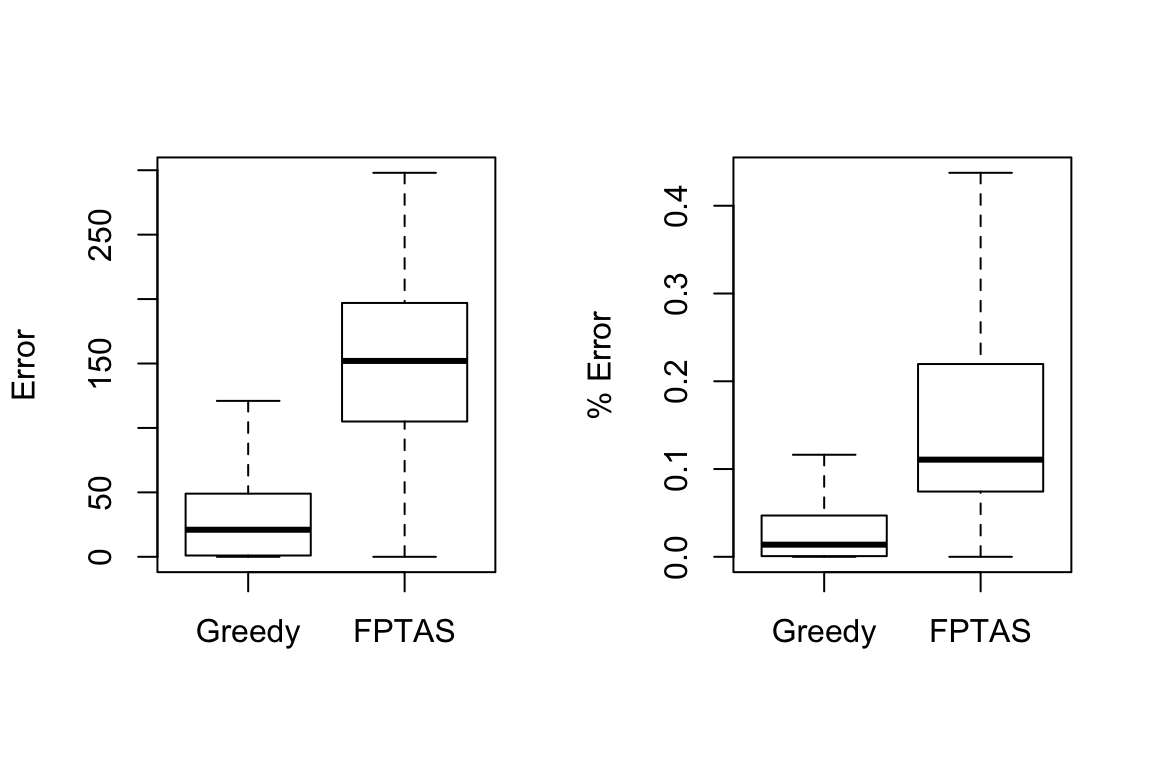
\includegraphics{report_files/figure-latex/plot-value-error-1} 

}

\caption{Error of FPTAS and Greedy algorithms}\label{fig:plot-value-error}
\end{figure}

Clearly, \textsc{FPTAS} does a lot worse than \textsc{Greedy}. This is
expected to us because \textsc{Greedy} is designed to obtain an optimal
value in 50\% range of the actual optimal value, while \textsc{FPTAS} is
designed to work for arbitrary precision--in this case, we set
\(\epsilon\) to 0.5 which should also guarantee values in 50\% range of
the optimal value. To see the range of error that each algorithm
produce, we can refer to the summary of percentage error below.

\begin{longtable}[]{@{}llllllll@{}}
\toprule
Name & Mean & Median & L.Quartile & U.Quartile & IQR & Min &
Max\tabularnewline
\midrule
\endhead
Greedy & 0.096 & 0.014 & 0.001 & 0.047 & 0.046 & 0 &
16.935\tabularnewline
FPTAS & 0.26 & 0.111 & 0.074 & 0.22 & 0.145 & 0 & 7.02\tabularnewline
\bottomrule
\end{longtable}

From both the plot and the table, we can see that both algorithms
actually do much better than expected, the percentage errors fall way
below 50\%. This might have to do with the way we \textbf{randomly}
generate the problem instances, since it is often the edge cases that
result in the 50\% error. Also, we can see that the maximum percentage
error produced by \textsc{FPTAS} is way less than that of
\textsc{Greedy}. This could be due to the mechanism of each algorithm.
In section \ref{algorithms}, we mentioned that \textsc{Greedy} has a
totally different approach to choosing the items and has a final step
where it might disregard previously obtained results and just choose the
item with maximum value; whereas \textsc{FPTAS} essentially uses
\textsc{MinCostDP} and its errors are due to the truncation while
scaling up and down the values of items, which potentially results in
smaller errors.

\section{Running Time}\label{running-time}

Next, we present the summary for the running time (milliseconds) of the
4 different algorithms.

\begin{longtable}[]{@{}llllllll@{}}
\toprule
Name & Mean & Median & L.Quartile & U.Quartile & IQR & Min &
Max\tabularnewline
\midrule
\endhead
MaxValDP & 142.861 & 63.797 & 14.824 & 209.059 & 194.235 & 0.036 &
941.761\tabularnewline
Greedy & 0.068 & 0.071 & 0.04 & 0.094 & 0.055 & 0.004 &
0.982\tabularnewline
MinCostDP & 392.519 & 249.554 & 56.087 & 660.346 & 604.258 & 0.181 &
1521.953\tabularnewline
FPTAS & 453.986 & 172.883 & 19.96 & 812.275 & 792.315 & 0.018 &
2175.657\tabularnewline
\bottomrule
\end{longtable}

These are just the summary of the result. Beside these, for each problem
instance, we also collect the number of items \(N\), the budget, and the
maximum value, as these might help us understand the running time
results better.

\begin{longtable}[]{@{}llllllll@{}}
\toprule
Name & Mean & Median & L.Quartile & U.Quartile & IQR & Min &
Max\tabularnewline
\midrule
\endhead
N & 355 & 355 & 180 & 530 & 350 & 10 & 700\tabularnewline
Budget & 88645 & 66829 & 25605 & 134347 & 108742 & 877 &
341526\tabularnewline
Max Value & 994 & 998 & 995 & 1000 & 5 & 642 & 1000\tabularnewline
\bottomrule
\end{longtable}

Through the running time summary alone, we can already see a general
trend in the running time. \textsc{Greedy} is the clear winner in terms
of speed. We have mentioned in section \ref{algorithms} that the running
time of \textsc{Greedy} is majorly contributed by the sorting step--the
choosing step after that is rather trivial. As such, the running time
depends on the input size, not the values of the items, not the budget.

\textsc{MaxValDP} has a significantly higher running time as compared to
that of \textsc{Greedy}. This is expected as we can see the in the
summary of instance information, the budget is much larger than the
number of instance.

Another observation is that \textsc{FPTAS} and \textsc{MinCostDP} have
almost similar running time. Again this can be explained by the fact
that \textsc{FPTAS} uses \textsc{MinCostDP} internally; i.e.
\textsc{FPTAS} takes slightly longer due to the scaling and trunscating
steps. Their running time, though, is almost 3 times as big as that of
\textsc{MaxValDP}. This totally depends on the choice of budget and the
maximum value of item in the problem instance.

\begin{figure}

{\centering 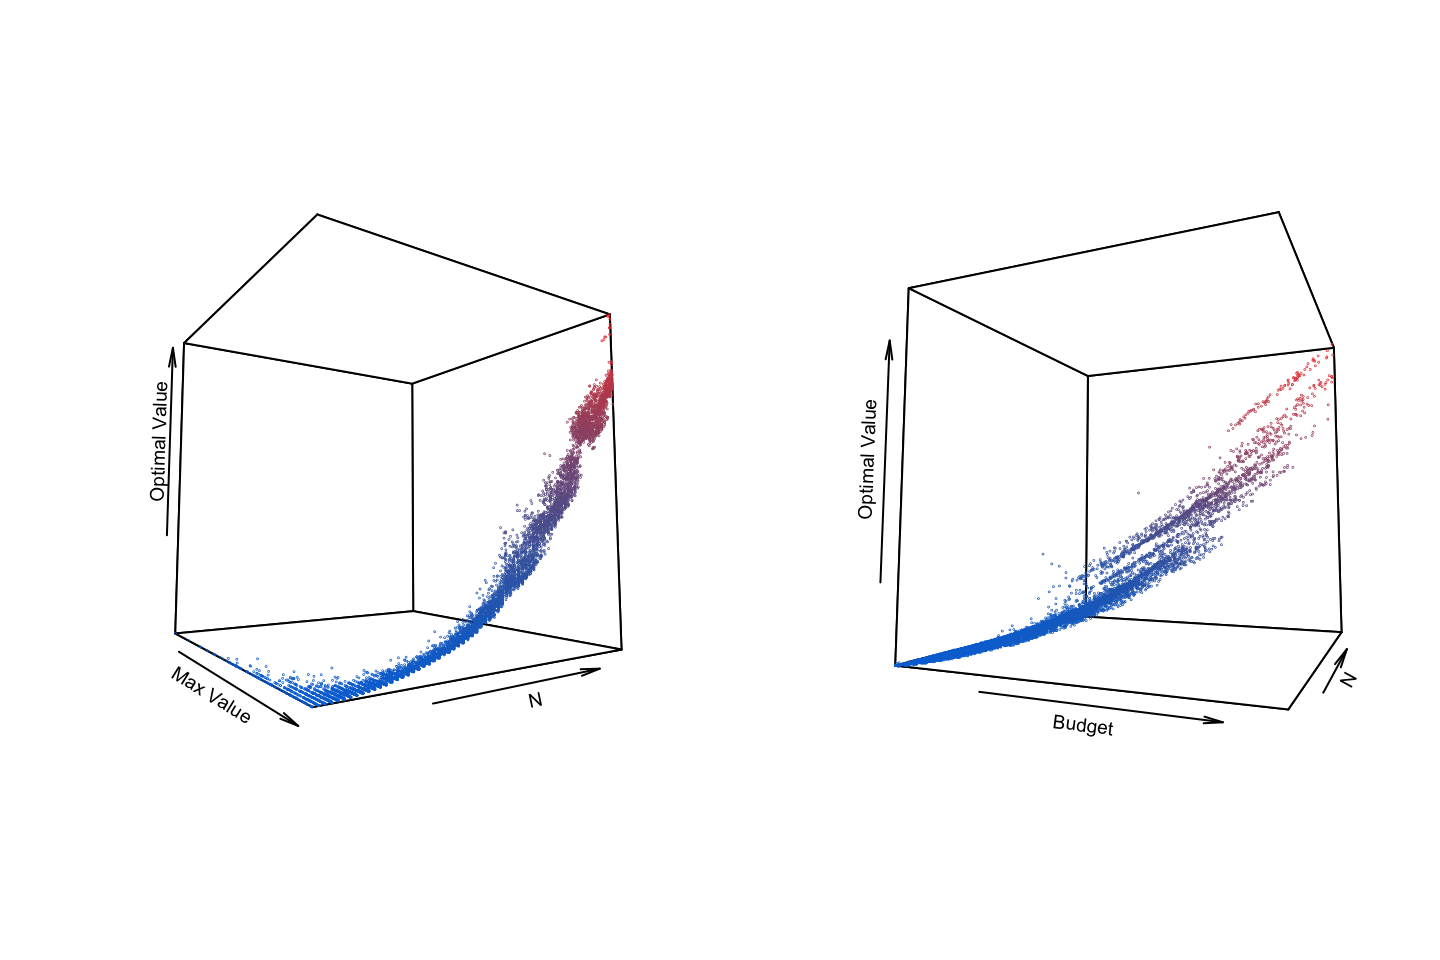
\includegraphics{report_files/figure-latex/plot-function-1} 

}

\caption{Running time of MinCostDP (left) and MaxValDP (right)}\label{fig:plot-function}
\end{figure}

Since we conduct the experiment with changing values of \(N\), we can
then make 3D plots of running time against \(N\) and the budget for
\textsc{MaxValDP} and running time against \(N\) and the maximum value
for \textsc{MinCostDP}. Refer to figure \ref{fig:plot-function}, for
\textsc{MinCostDP}, based on the curvature of the plot surface, we can
see that the relationship between \(N\) and the optimal value is clearly
non-linear, in fact, we can even see that it is indeed quadratic as the
theory suggested. Whereas, for \textsc{MaxValDP}, we can see that the
budget and \(N\) seem to be linearly related to the optimal value.

\chapter{Conclusion}\label{conclusion}

We can come up with the conclusion that \textsc{MaxValDP}, the vanilla
flavor, shows why it is generally favored. It guarantees the optimal
value (with 100\% accuracy) and relatively acceptable running time. The
versatile \textsc{FPTAS} actually does worse in both aspect, accuracy
and running time; but to do justice to it, it shines for its
versatility; as compared to other approximation method which targets a
specific range of error, e.g. \textsc{Greedy}, it will not perform as
good, otherwise, we will deem \textsc{Greedy} as useless and get rid of
it. \textsc{Greedy}, though, runs amazingly fast and yields acceptable
accuracy. The last flavor, \textsc{MinCostDP} is like chocolate. Hardly
can anyone argue whether chocolate or vanilla is ultimately the better
flavor. Perhaps, even on situational basis: it is actually pretty hard
to come up with an example to show that a type of pastries must come
with chocolate instead of vanilla \ldots{} apparently brownies can also
come with vanilla. We guess the moral of the story is not that you can
use either dynamic programming approach to solve any Maximum 0-1
Knapsack problem, but some go better with \textsc{MaxValDP} and others
go better with \textsc{MinCostDP}, such as those problems with really
high maximum value.

\bibliography{packages.bib,book.bib}

\end{document}
